


The Chang'E-4 mission, initiated at the end of 2018, coincided with a period of solar activity minimum characterized by a scarcity of \ac{SEP} events. However, as the Sun entered the increase phase of new \ac{SC} and become more active than the solar activity minimum, solar activity intensified, and consequencely, a growing number of \ac{SEP} events, including prolonged-duration and high-intensity ones, were observed to reach the lunar surface and were detected by the \ac{LND} on the lunar far-side surface. For example, \citet{Guo2023GRL} recently reported the first \ac{GLE} of \ac{SC} 25, which was concurrently detected by instruments deployed on the Moon, Earth, Mars and also by \ac{SolO} as well as \ac{PSP} \citep{Papaioannou2022AA, Martucci2023SpWea, Chertok2022MNRAS}. It is noteworthy that \ac{LND} was switched on after the initial phase of the event, hence did not cover the whole event. Even so, it still advances our understanding of potential radiaton risks that are caused by these extreme \ac{SEP} events on the surface of solar system bodies.
In the appendix section of this thesis, a comprehensive list of \ac{SEP} events detected by \ac{LND} on the lunar far-side surface between 2019 and 2023 is provided, further emphsizing \ac{LND}'s contribution to the study of \acs{SEP}.


The \ac{SEP} event on May 6, 2019 is the first \ac{SEP} event that has ever been detected on the lunar surface, according to our knowledge. 
This \ac{SEP} event is associated with an M-class flare originating from a solar active region (AR12470) which is located in the eastern hemisphere and is more than 110 degrees away from the Earth's magnetic footpoint on the solar surface. The remote-sensing observations conducted by the \ac{SOHO}/\ac{LASCO} and the \ac{STEREO} revealed the presence of a slow, narrow, and westward moving \ac{CME}. 
Though the \acp{SEP} from this event cause negligible radiation dose due to its weak intensity and lower peak energy, it is still an interesting event and worth studying due to the following two reasons.
The primary objective of this study is to utilize the first \ac{SEP} event observed by \ac{LND} to validate the data products produced during \ac{SEP} occurrences and assess the instrument's performance under such conditions. By cross calibrating the proton measurements between \ac{LND} and other already existed particle instruments at \ac{L1} , such as the \ac{EPHIN} onboard \ac{SOHO} and the \ac{EPAM} onboard \ac{ACE}, we conclude that \ac{LND} provides reliable solar energetic proton measurement with a good time resolution of one minute.
%For sure LND is outside of the mangetosphere, but still that is one of the thing worth to look at. How the SEP propogarting across the magnetosphere and arrive the magnetosphere tails.
In addition, we investigate the extensive spatial distributions of this \ac{SEP} by using both in-situ and remote-sensing measurements. Unlike the typical widespread \ac{SEP} events which persist for few days and are accompanied with broad \ac{CME}, the temporal profile of this event and remote-sensing observation imply that it is an impulsive event that has good magnetic connections. Several mechanisms could be involved in the process of the particle traversal across considerable distance in the so-call wide spread \acs{SEP}. 
%Combined the in-site and remote-sensing measurement, we try to found out what kind release and propagation mechanism are involved in this event.

\subsection*{Short Overview of the publication}

First, we check and analyze the in-situ data from May 3, 2019 to May 8, 2019 in detail fron different view points and different detectors. Proton and electron flux, solar wind parameters and local magnetic field measured at \ac{L1} are given.
Though \ac{STEREO}-A had better magnetic connection, the background on \ac{STEREO}-A is dominated by particles from a pre-existing \ac{SEP} and is therefore not included here in analysis.
Then we determine the onset time based on the combined data from \ac{LND}, \ac{EPHIN}, \ac{EPAM} and \acs{3DP}. A Poisson-CUSUM method \citep{Huttunen2005AA, Palmroos2022FrASS} which refers to a cumulative sum method for variables that follow Poisson distribution is applied to tackle the lower statistic measurements. By fitting the velocity dispersion, we derived the release time of protons and electrons. Besides, the proton integral spectra of the \ac{SEP} event is also derived. In the end of the observation section, we analyze the remote-sensing observation including X-ray flux, radio observation \ac{CME} and EUV waves observations. This work attempts to answer questions S1 and S2 regarding \acp{SEP}.


The key observations of the publication are:
\begin{itemize}
    \item \ac{LND} has consistent measurements with other \ac{L1} instruments during the first \ac{SEP} events, including the consistent onset time and spectra.
    \item Protons and electrons have show clearly velocity dispersion and are beam-like structures. The release time of electrons is an hour earlier than that of protons.
    \item The magnetic footpoint of Earth is about 113$^\circ$ away from the flare location. The accompanied \ac{CME} is slow and narrow. We found no evidence of EUV arrival at the magnetic footpoint of Earth. 
    \item The more than 100 degree longitudinal seperation is hard to explain in an impulsive \ac{SEP} event. Possible reasons include the expanding coronal shock, irregular magnetic field, and magnetic field line random walk, or the mixture of the above three. Besides, the release mechanism of electrons and protons might be different due to their distinct behaviors.
\end{itemize}

The following article is reproduced from \textcite{Xu2020ApJ} by permission of the AAS:\\

\noindent\pubcite{Xu2020ApJ}\\
\strut\hfill Own contribution: 90\%

\newpage
\newcounter{includepdfpageAPJLTwenty}

\addtocounter{section}{1}
\setcounter{section}{1} 
% \phantomsection
% \addcontentsline{toc}{section}{\arabic{chapter}.\arabic{section} First Solar Energetic Particles Measured on the Lunar Far-side(Publication ApJ Letter 2020)}
%
\phantomsection
\addcontentsline{toc}{section}{\arabic{chapter}.\arabic{section} Introduction}
\label{sec:paper_xu2020}
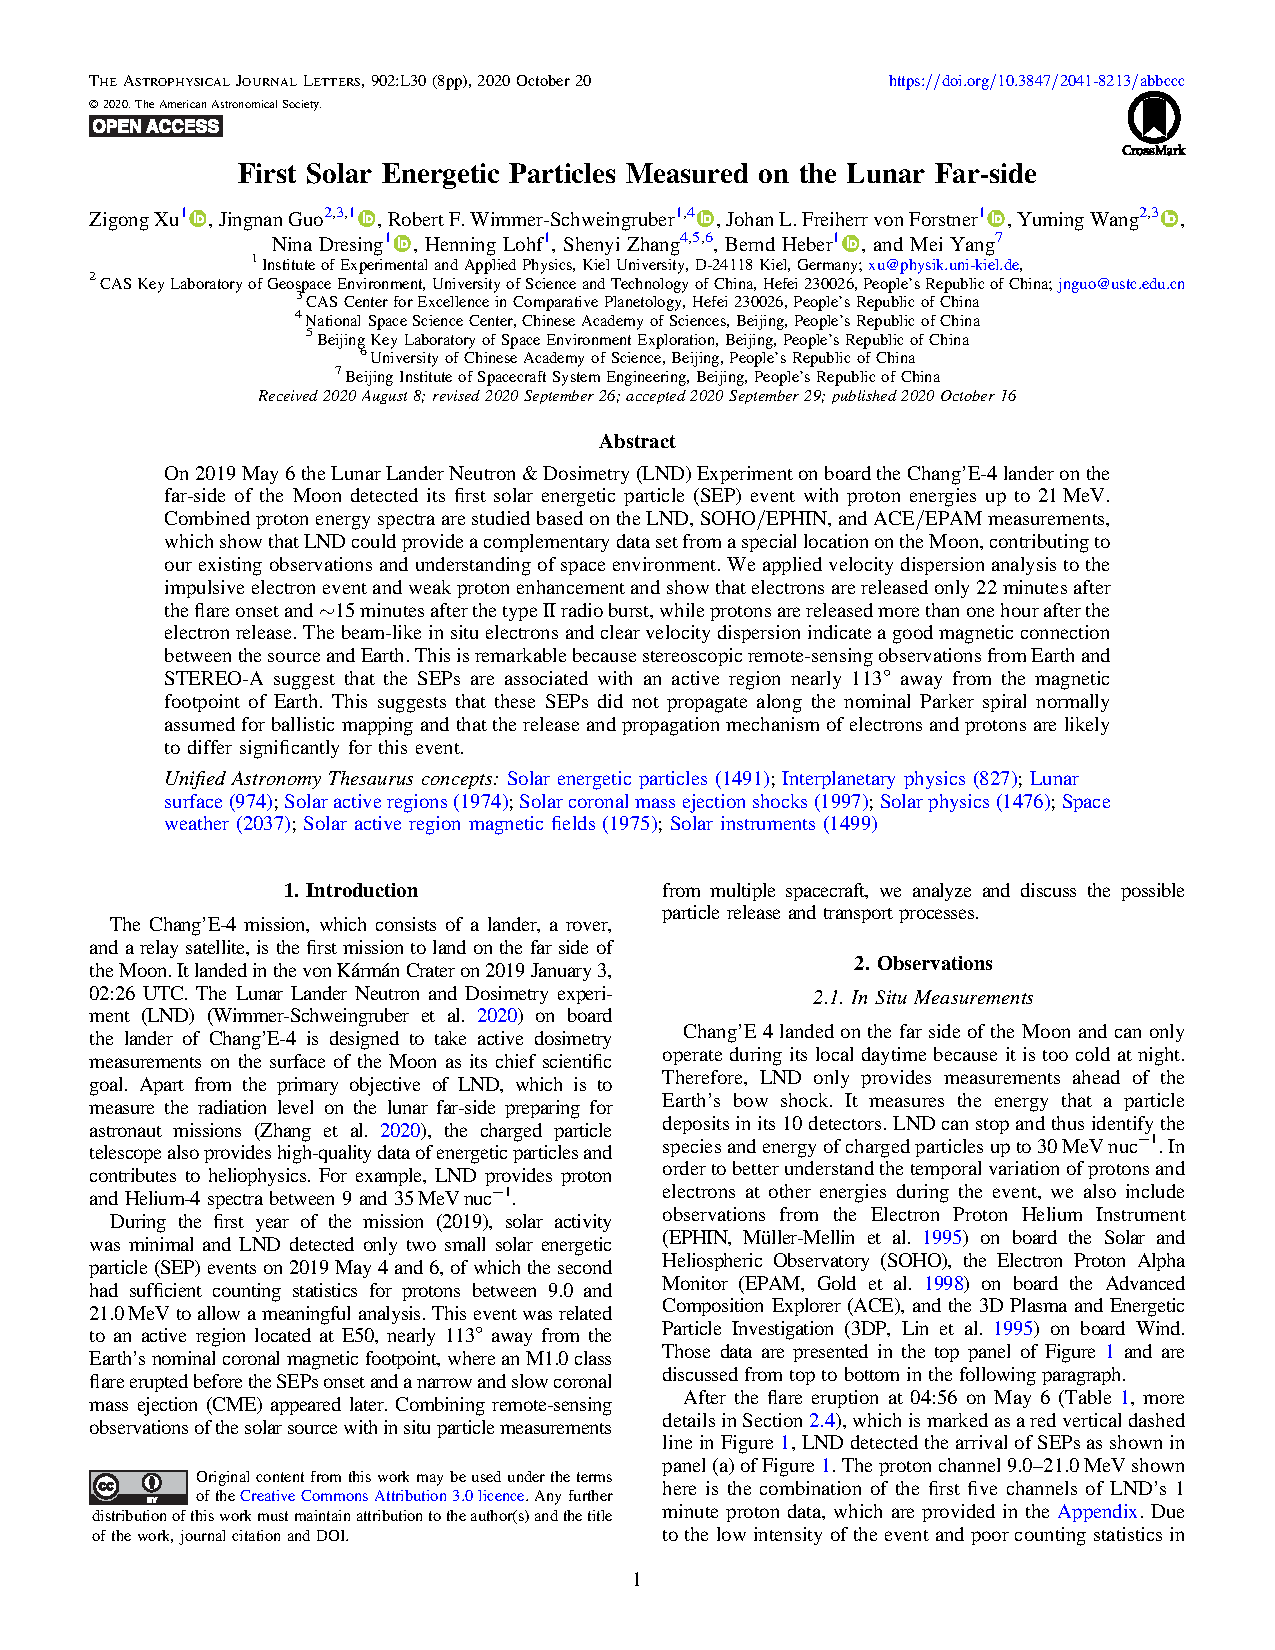
\includepdf[pages={1}, link, linkname=paper_xu2020, scale=.9, pagecommand={\refstepcounter{includepdfpageAPJLTwenty}\label{paper_xu2020.\theincludepdfpageAPJLTwenty}}]{publications/Xu_et_al_2020_ApJL.pdf}
%
\addtocounter{section}{1} 
\phantomsection
\addcontentsline{toc}{section}{\arabic{chapter}.\arabic{section} Observations}
\includepdf[pages={2-4}, link, linkname=paper_xu2020, scale=.9, pagecommand={\refstepcounter{includepdfpageAPJLTwenty}\label{paper_xu2020.\theincludepdfpageAPJLTwenty}}]{publications/Xu_et_al_2020_ApJL.pdf}
%
\addtocounter{section}{1} 
\phantomsection
\addcontentsline{toc}{section}{\arabic{chapter}.\arabic{section} Summary and Discussion}
\includepdf[pages={5-6}, link, linkname=paper_xu2020, scale=.9, pagecommand={\refstepcounter{includepdfpageAPJLTwenty}\label{paper_xu2020.\theincludepdfpageAPJLTwenty}}]{publications/Xu_et_al_2020_ApJL.pdf}
%
\addtocounter{section}{1} 
\phantomsection
\addcontentsline{toc}{section}{\arabic{chapter}.\arabic{section} Appendix}
\includepdf[pages={7}, link, linkname=paper_xu2020, scale=.9, pagecommand={\refstepcounter{includepdfpageAPJLTwenty}\label{paper_xu2020.\theincludepdfpageAPJLTwenty}}]{publications/Xu_et_al_2020_ApJL.pdf}
%
\addtocounter{section}{1} 
\phantomsection
\addcontentsline{toc}{section}{\arabic{chapter}.\arabic{section} References}
\includepdf[pages={8}, link, linkname=paper_xu2020, scale=.9, pagecommand={\refstepcounter{includepdfpageAPJLTwenty}\label{paper_xu2020.\theincludepdfpageAPJLTwenty}}]{publications/Xu_et_al_2020_ApJL.pdf}
